% OpenMarket systems paper — LaTeX entry point
% Build:  ./scripts/compile.sh   (generates figures, then latexmk)
% Clean:  latexmk -C

\documentclass[11pt,a4paper]{article}

\usepackage[T1]{fontenc}
\usepackage[utf8]{inputenc}
\usepackage{lmodern}
\usepackage{microtype}
\usepackage{amsmath,amssymb}
\usepackage{graphicx}
\usepackage{booktabs}
\usepackage{placeins}
\usepackage{xurl}
\usepackage{hyperref}
\usepackage{url}
\setlength{\emergencystretch}{2em}
\usepackage{listings}
\usepackage{upquote}
\usepackage{xcolor}
\usepackage{tikz}
\usetikzlibrary{arrows.meta,positioning,calc,shapes.geometric}

% Shared flowchart styles (TikZ replaces matplotlib pipeline diagrams)
\tikzset{
  flowbox/.style={
    rectangle, rounded corners=2pt, draw=blue!45!black,
    fill=blue!6, align=center, inner sep=4pt,
    minimum width=2.55cm, minimum height=0.72cm, font=\small
  },
  narrowbox/.style={
    flowbox, minimum width=2.05cm, minimum height=0.62cm, font=\footnotesize
  },
  widebox/.style={
    flowbox, minimum width=2.15cm
  },
  flowarr/.style={
    -{Stealth[length=2.2mm]}, semithick, draw=black!70
  }
}

\usepackage[numbers,sort&compress]{natbib}
\bibliographystyle{plainnat}

\hypersetup{
  colorlinks=true,
  linkcolor=blue,
  citecolor=blue,
  urlcolor=blue,
  pdftitle={OpenMarket: A Synchronized Polymarket--Binance Dataset for High-Frequency Prediction-Market Research},
  pdfauthor={Gregory Young}
}

\graphicspath{{assets/figures/}}

\lstset{
  basicstyle=\ttfamily\footnotesize,
  breaklines=true,
  breakatwhitespace=true,
  columns=fullflexible,
  keepspaces=true,
  showstringspaces=false,
  frame=single,
  backgroundcolor=\color{gray!8}
}

\title{%
  OpenMarket: A Synchronized Polymarket--Binance\\
  Dataset for High-Frequency Prediction-Market Research
}

\author{%
  Gregory Young\\
  Department of Computer Science\\
  University of Colorado Boulder\\
  Boulder, CO 80309\\
  \texttt{gryo8540@colorado.edu}
}

\date{\today}

% Auto-generated stats (scripts/paper/analyze_unified.py)
\IfFileExists{assets/stats/characterization.tex}{
  % Auto-generated by scripts/paper/analyze_unified.py — do not edit by hand
\newcommand{\OpenMarketReleaseTag}{v0.5.2}
\newcommand{\OpenMarketTotalRows}{727,098,247}
\newcommand{\OpenMarketUnifiedGiB}{8.69}
\newcommand{\OpenMarketSnapshots}{202}
\newcommand{\OpenMarketLagPairs}{2,936,031}
\newcommand{\OpenMarketLagMedian}{16}
\newcommand{\OpenMarketLagPFive}{-186}
\newcommand{\OpenMarketLagPNinetyFive}{316}
\newcommand{\OpenMarketUnifiedMetaScanSeconds}{0.118}
\newcommand{\OpenMarketLagPairsLoadSeconds}{0.018}
\newcommand{\OpenMarketCollectionStart}{2026-03-14}
\newcommand{\OpenMarketCollectionEnd}{2026-07-01}
\newcommand{\OpenMarketRustLoc}{17,824}
\newcommand{\OpenMarketPolyObservedDays}{54}
\newcommand{\OpenMarketBinanceObservedDays}{57}
\newcommand{\OpenMarketDataFirstDay}{2026-02-12}
\newcommand{\OpenMarketDataLastDay}{2026-05-15}
\newcommand{\OpenMarketDataSpanDays}{93}
\newcommand{\OpenMarketHardware}{Apple M5 Max, 64~GB RAM}
\newcommand{\OpenMarketRustVersion}{rustc 1.94.0 (4a4ef493e 2026-03-02) (Homebrew)}
\newcommand{\OpenMarketBenchHfLoad}{0.002}
\newcommand{\OpenMarketBenchFeatLoad}{0.0052}
\newcommand{\OpenMarketBenchFeatRows}{33,349}
\newcommand{\OpenMarketBenchFeatParts}{3}
\newcommand{\OpenMarketBenchBacktest}{0.09}
\newcommand{\OpenMarketBenchBacktestMarkets}{89}
\newcommand{\OpenMarketFeatureCorrRows}{33,084}
\newcommand{\OpenMarketFeatureCorrFeatures}{18}

}{
  \newcommand{\OpenMarketReleaseTag}{v0.5.2}
  \newcommand{\OpenMarketTotalRows}{727,098,247}
  \newcommand{\OpenMarketUnifiedGiB}{8.69}
  \newcommand{\OpenMarketSnapshots}{202}
  \newcommand{\OpenMarketLagPairs}{2,936,031}
  \newcommand{\OpenMarketLagMedian}{16}
  \newcommand{\OpenMarketLagPFive}{-186}
  \newcommand{\OpenMarketLagPNinetyFive}{316}
  \newcommand{\OpenMarketCollectionStart}{2026-03-14}
  \newcommand{\OpenMarketCollectionEnd}{2026-07-01}
  \newcommand{\OpenMarketRustLoc}{17,823}
  \newcommand{\OpenMarketPolyObservedDays}{54}
  \newcommand{\OpenMarketBinanceObservedDays}{57}
  \newcommand{\OpenMarketDataFirstDay}{2026-02-12}
  \newcommand{\OpenMarketDataLastDay}{2026-05-15}
  \newcommand{\OpenMarketDataSpanDays}{93}
}

% Auto-generated research macros (scripts/paper/analyze_research.py)
\IfFileExists{assets/stats/research_stats.tex}{
  % Auto-generated by analyze_research.py — do not edit by hand
\newcommand{\OpenMarketAucDiff}{0.0014}
\newcommand{\OpenMarketAucDiffLow}{0.0013}
\newcommand{\OpenMarketAucDiffHigh}{0.0015}
\newcommand{\OpenMarketAucPvalue}{<0.001}
\newcommand{\OpenMarketLogisticEce}{0.027}
\newcommand{\OpenMarketNaiveEce}{0.014}
\newcommand{\OpenMarketLogisticScoreUs}{0.087}
\newcommand{\OpenMarketBrierTight}{0.162}
\newcommand{\OpenMarketBrierWide}{0.185}
\newcommand{\OpenMarketLagPriceCorr}{0.00}

}{
  \newcommand{\OpenMarketAucDiff}{0.0014}
  \newcommand{\OpenMarketAucDiffLow}{0.0013}
  \newcommand{\OpenMarketAucDiffHigh}{0.0015}
  \newcommand{\OpenMarketAucPvalue}{<0.001}
  \newcommand{\OpenMarketLogisticAuc}{0.8415}
  \newcommand{\OpenMarketNaiveAuc}{0.8401}
  \newcommand{\OpenMarketDriftAuc}{0.7725}
  \newcommand{\OpenMarketImbalanceAuc}{0.5863}
  \newcommand{\OpenMarketBrierTight}{0.161}
  \newcommand{\OpenMarketBrierWide}{0.184}
  \newcommand{\OpenMarketSpreadMedian}{0.01}
  \newcommand{\OpenMarketSpreadPNinety}{0.01}
  \newcommand{\OpenMarketSpreadPNinetyFive}{0.02}
  \newcommand{\OpenMarketSpreadPNinetyNine}{0.03}
  \newcommand{\OpenMarketSpreadOneTickPct}{91.9}
  \newcommand{\OpenMarketSpreadTwoTickPct}{6.0}
  \newcommand{\OpenMarketLagPriceCorr}{0.00}
  \newcommand{\OpenMarketLogisticEce}{0.027}
  \newcommand{\OpenMarketNaiveEce}{0.015}
  \newcommand{\OpenMarketLogisticScoreUs}{0.102}
  \newcommand{\OpenMarketBootstrapN}{2,000}
  \newcommand{\OpenMarketOosRows}{355,814}
  \newcommand{\OpenMarketNaiveOosAuc}{0.8405}
  \newcommand{\OpenMarketNaiveOosBrier}{0.163}
  \newcommand{\OpenMarketNaiveOosEce}{0.014}
  \newcommand{\OpenMarketNaiveOosLogLoss}{0.485}
  \newcommand{\OpenMarketModelOosAuc}{0.8378}
  \newcommand{\OpenMarketModelOosBrier}{0.165}
  \newcommand{\OpenMarketModelOosEce}{0.025}
  \newcommand{\OpenMarketModelOosLogLoss}{0.495}
  \newcommand{\OpenMarketFlagTightPct}{67.6}
  \newcommand{\OpenMarketFlagMediumPct}{27.0}
  \newcommand{\OpenMarketFlagWidePct}{5.5}
  \newcommand{\OpenMarketEnvBinanceMed}{99}
  \newcommand{\OpenMarketEnvBinanceRange}{4}
  \newcommand{\OpenMarketEnvPolyMed}{7}
  \newcommand{\OpenMarketEnvPolyRange}{2}
  \newcommand{\OpenMarketDriftBound}{6}
  \newcommand{\OpenMarketJumpCount}{15,148}
  \newcommand{\OpenMarketJumpMatched}{4,272}
  \newcommand{\OpenMarketRespMedianIngest}{347}
  \newcommand{\OpenMarketRespMedianSource}{345}
  \newcommand{\OpenMarketDelayAsym}{97}
}

\begin{document}
\maketitle

\begin{abstract}
OpenMarket began as an attempt to trade Polymarket's BTC 15-minute binary
markets against Binance BTC/USDT order flow. The attempt did not produce a
tradable edge: out-of-sample, a walk-forward logistic model over 43
microstructure features matches but does not beat the probability already
implied by Polymarket's own order book, and simulated trading nets
$-0.117$ per trade under stated fee and slippage assumptions. We release
the synchronized corpus and infrastructure that attempt produced---to our
knowledge, the first public millisecond-level Polymarket BTC / Binance
BTC-USDT paired corpus with explicit pairing metadata. The frozen archive
(tag \OpenMarketReleaseTag{}) contains
\OpenMarketTotalRows{} deduplicated rows across \OpenMarketSnapshots{}
archival snapshots, with event data on \OpenMarketPolyObservedDays{}
observed days between \OpenMarketDataFirstDay{} and
\OpenMarketDataLastDay{}, including \OpenMarketLagPairs{} explicit
lead--lag pairs, alongside a reproducible Rust pipeline for collection,
millisecond pairing, Parquet export, and walk-forward calibration. Initial
analyses establish Polymarket stylized facts (one-tick top-of-book spreads)
and characterize cross-venue timing: an apparent \OpenMarketLagMedian{}~ms
median lag on venue source clocks, with relative clock drift bounded to
${\leq}\OpenMarketDriftBound{}$~ms over the archive but a remaining
single-vantage constant-offset ambiguity of roughly
$\pm\OpenMarketEnvBinanceMed{}$~ms. A synchronization-free event study, measured
only on the collector clock, independently shows that Polymarket quotes
respond to large Binance moves after a median \OpenMarketRespMedianIngest{}~ms.
We position this work as a data-and-methods release whose central empirical
result is an honest null.
\end{abstract}

\section{Introduction}
\label{sec:introduction}

OpenMarket began as a trading system, not a dataset. We built a Rust
pipeline to trade Polymarket's BTC 15-minute binary markets against Binance
BTC/USDT spot flow: WebSocket collectors for both venues, a millisecond
recorder, a walk-forward calibrated logistic scorer, and simulated and paper
execution. The result was negative. No strategy iteration survived fees and
spread; out-of-sample, the strongest published model \emph{does not beat, and
slightly underperforms} the probability already implied by Polymarket's own
order book (Section~\ref{sec:insights-forecast}); and simulated positive-EV
trading nets $-0.116$ normalized payoff units per attempted trade under stated
fee and slippage assumptions. We do not claim trading profitability---the
central empirical finding is the opposite, and that negative result is
published with the data that produced it.

This paper releases the resulting infrastructure and corpus, which outlived
the trading strategy. Empirical work now documents tick-level
Polymarket dynamics, decentralized prediction-market (DePM) design
trade-offs, and combinatorial arbitrage
\cite{dubach2026anatomy,saguillo2025arbitrage,rahman2025sok}. What remains
missing is a \textbf{public, cross-venue, millisecond-resolution corpus}
paired with Binance BTC/USDT and tooling that makes synchronization
quality, lead--lag, and calibration analysis reproducible at archival
scale. OpenMarket closes that gap. The contribution is threefold:
\begin{enumerate}
  \item \textbf{Corpus.} To our knowledge, the first public millisecond-level
        Polymarket BTC / Binance BTC-USDT paired corpus with explicit pairing
        metadata: \OpenMarketTotalRows{} deduplicated rows across
        \OpenMarketSnapshots{} archival snapshots, with event data on
        \OpenMarketPolyObservedDays{} observed days
        (\OpenMarketDataFirstDay{}--\OpenMarketDataLastDay{};
        Section~\ref{sec:exp-scale}), including
        \OpenMarketLagPairs{} explicit lead--lag pairs.
  \item \textbf{Methods.} Documented source-vs.-ingest synchronization
        with empirical clock-offset validation
        (Section~\ref{sec:sync-clock}), Parquet-native export,
        walk-forward calibration training, and validation harnesses that
        treat clock drift and pairing-window sensitivity as measurable
        objects rather than implementation details.
  \item \textbf{Empirical baselines.} Stylized facts and forecast
        benchmarks on the released corpus---top-of-book spreads, lead--lag
        distributions, and ablations testing whether multivariate models
        outperform naive order-book mid priors (out-of-sample, they do
        not).
\end{enumerate}

The initial empirical claims are intentionally narrow:
\begin{enumerate}
  \item BTC 15-minute top-of-book spreads are usually one tick wide.
  \item Source-clock lead--lag has a compact median but heavy tails.
  \item Polymarket quotes respond to large Binance moves after hundreds of
        milliseconds on the collector clock.
  \item Lead--lag timing changes little across cross-venue disagreement regimes.
  \item Multivariate features slightly underperform the Polymarket mid prior
        out-of-sample.
\end{enumerate}

The released artifacts deliberately include the full research trail: the
collectors and recorder, the synchronization layer, the feature and
training pipelines, the backtesting framework, the strategy-evolution archive,
the Hugging Face dataset and model releases, and a sanitized operational
appendix for audit context. OpenMarket is frozen as a public research archive
(source tag \OpenMarketReleaseTag{}); active collection has ended. The remainder of the
paper describes the system, the released artifacts, and initial microstructure
findings that prior single-venue or closed pipelines cannot support.

\section{Background}
\label{sec:background}

Prediction markets aggregate information through prices of contracts tied to
future outcomes~\cite{wolfers2004prediction,hanson2003combinatorial}. Polymarket
lists binary outcome markets where contracts settle to 1 if an event occurs and 0
otherwise. BTC 15-minute markets ask whether Bitcoin will be above or below a
reference price at the end of a short window. These markets combine elements of
options, sports-style binary markets, and crypto exchange microstructure.
Recent Polymarket microstructure and DePM surveys are summarized in
Section~\ref{sec:related-work}. Reproducible public infrastructure for
high-frequency cross-venue work remains scarce.

Binance BTC/USDT serves as the reference stream because it is liquid,
high frequency, and tied to the Polymarket BTC settlement window. Following
multi-venue price-discovery practice~\cite{hasbrouck1995one}, we align Binance
trades with Polymarket book updates, derive features, generate labels, and
evaluate models without leaking future information. Millisecond-resolution
storage and pairing follow standard high-frequency microstructure
practice~\cite{ohara2015high,cont2014price}.
\section{Related Work}
\label{sec:related-work}

Prediction markets aggregate dispersed information into tradable prices
\cite{wolfers2004prediction,hanson2003combinatorial,berg2008prediction}.
High-frequency microstructure methods emphasize order-book dynamics, latency,
and price impact \cite{ohara2015high,cont2014price}. Multi-venue studies
measure which market contributes to price discovery \cite{hasbrouck1995one},
and cross-exchange price dislocations in crypto markets are documented at
scale by Makarov and Schoar~\cite{makarov2020trading}.

\textbf{Public high-frequency order-book datasets.}
LOBSTER~\cite{huang2011lobster} reconstructs NASDAQ limit-order books for
academic use, and FI-2010~\cite{ntakaris2018benchmark} is a widely used
mid-price forecasting benchmark; both cover traditional equity venues.
OpenMarket follows this lineage but targets a decentralized prediction-market
CLOB paired with a crypto spot reference stream, with explicit cross-venue
pairing metadata.

\textbf{Polymarket microstructure.}
Dubach~\cite{dubach2026anatomy} analyzes tick-level Polymarket order-book
evidence and releases analysis code, but does not ship a synchronized Binance
reference stream or a Hugging Face archival corpus. Saguillo et al.~\cite{saguillo2025arbitrage}
document combinatorial arbitrage and market replications using proprietary-scale
scrapes; reproduction requires re-implementing data collection. Rahman et al.~\cite{rahman2025sok}
survey DePM design trade-offs without a cross-venue BTC 15-minute benchmark.

\textbf{Crypto spot data.}
Public Binance kline and aggTrade products are widely used, but they do not
include Polymarket CLOB state, settlement labels, or pairing metadata needed for
prediction-market forecasting studies.

\textbf{Open infrastructure.}
Most open-source trading repositories mix notebooks, private snapshots, and
undocumented assumptions. OpenMarket differs by publishing (i) raw and deduped
Parquet splits, (ii) explicit \texttt{lag\_pairs\_ms} with quality flags, (iii)
Rust exporters/trainers with pinned commands, and (iv) empirical baselines on the
released corpus.

We claim infrastructure and reproducible characterization, not superior live
trading performance. Dubach provides a deeper single-venue microstructure
analysis, while Saguillo et al. study broader proprietary-scale arbitrage data
than this public BTC 15-minute release.

\section{System Architecture and Data Collection}
\label{sec:architecture}

\begin{figure}[t]
  \centering
  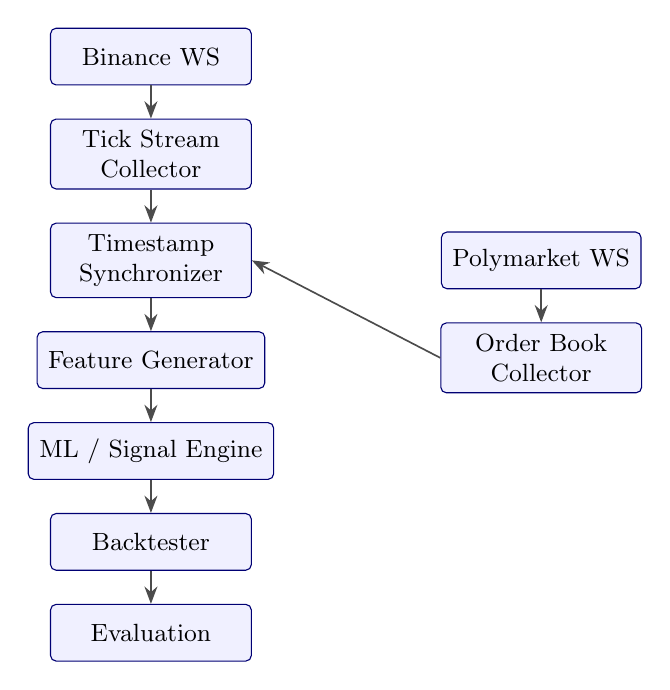
\begin{tikzpicture}[
      node distance=0.42cm,
      every node/.style={flowbox}
    ]
    \node (bws) {Binance WS};
    \node[below=of bws] (tick) {Tick Stream\\Collector};
    \node[below=of tick] (sync) {Timestamp\\Synchronizer};
    \node[below=of sync] (feat) {Feature Generator};
    \node[below=of feat] (ml) {ML / Signal Engine};
    \node[below=of ml] (bt) {Backtester};
    \node[below=of bt] (eval) {Evaluation};

    \node[right=2.4cm of sync, minimum width=2.2cm] (pws) {Polymarket WS};
    \node[below=of pws] (book) {Order Book\\Collector};

    \draw[flowarr] (bws) -- (tick);
    \draw[flowarr] (tick) -- (sync);
    \draw[flowarr] (sync) -- (feat);
    \draw[flowarr] (feat) -- (ml);
    \draw[flowarr] (ml) -- (bt);
    \draw[flowarr] (bt) -- (eval);
    \draw[flowarr] (pws) -- (book);
    \draw[flowarr] (book.west) -- (sync.east);
  \end{tikzpicture}
  \caption{OpenMarket pipeline. Binance and Polymarket WebSocket streams feed
    collectors; the recorder synchronizes events and exports aligned tables for
    feature generation, signals, and backtesting.}
  \label{fig:architecture}
\end{figure}

The codebase is a Rust workspace spanning exchange collectors, a multi-market
recorder with lag-pairing export, signal and execution engines, backtesting, and
Parquet-native ML crates (\texttt{step3-parquet-export},
\texttt{binary-outcome-trainer}); Figure~\ref{fig:architecture} shows how the
two WebSocket streams converge on the synchronizer and downstream stages.
Crate-level detail is maintained in the repository; the paper's benchmark
claims are regenerated from the frozen dataset and model artifacts, not from
live operational services.

\subsection{Binance}
\label{sec:data-binance}

The Binance collector records BTC/USDT trades and derives candle tables at
multiple time resolutions. The source schema includes trade ID, trade timestamp,
price, quantity, quote volume, maker/taker direction, and local receive time.
Millisecond-level tick snapshots preserve both source and ingest timestamps.

\subsection{Polymarket}
\label{sec:data-polymarket}

The Polymarket collector subscribes to BTC binary market order book updates,
trades, and last-trade-price events. The recorder maps token IDs to market slugs
and side labels using market metadata so that UP and DOWN books can be analyzed
consistently across rolling 15-minute markets.

\subsection{Storage}
\label{sec:data-storage}

The initial recorder stores data in SQLite for operational simplicity. The
public dataset release exports raw and processed tables to partitioned Parquet.
Key recorded tables include:
\begin{itemize}
  \item \texttt{binance\_trades}, \texttt{binance\_ticks\_ms}
  \item \texttt{polymarket\_ticks\_ms}, \texttt{market\_meta}
  \item \texttt{lag\_pairs\_ms}
  \item \texttt{binance\_candles\_1s}, \texttt{binance\_candles\_5s},
        \texttt{binance\_candles\_1m}, \texttt{binance\_candles\_5m},
        \texttt{binance\_candles\_15m}, \texttt{binance\_candles\_1h}
\end{itemize}

% Included from main.tex via % Included from main.tex via % Included from main.tex via \input{sections/synchronization}

\section{Synchronization}
\label{sec:synchronization}

Synchronization is the central technical component of OpenMarket.
For each event the recorder stores both a source timestamp (exchange-emitted)
and an ingest timestamp (collector-observed):
\begin{align}
  \texttt{source\_ts\_ms} &= \text{timestamp from the exchange or event source}, \\
  \texttt{ingest\_ts\_ms}  &= \text{timestamp when the collector received the event}.
\end{align}
Following multi-venue price-discovery practice~\cite{hasbrouck1995one},
we pair Binance and Polymarket observations inside a bounded millisecond
window and compute lead-lag as
\begin{equation}
  \texttt{lead\_lag\_ms}
    = \texttt{polymarket\_source\_ts\_ms} - \texttt{binance\_source\_ts\_ms}.
  \label{eq:lead-lag}
\end{equation}
Positive values indicate that the Polymarket event timestamp follows the
Binance event timestamp; negative values indicate the opposite.
Each pair is stored with a quality flag, Binance price, Polymarket bid,
market slug, side label, and price delta in basis points.

\subsection{Pairing and Quality Metrics}

The recorder pairs events when their source timestamps fall within a
configurable alignment window~$W$ (milliseconds).
OpenMarket treats the following as first-class dataset quality metrics,
consistent with microstructure guidance for decentralized prediction
markets~\cite{dubach2026anatomy,rahman2025sok}:
clock drift, dropped WebSocket messages, duplicate payloads, reconnect gaps,
stale order-book state, out-of-order events, and sensitivity to~$W$.

\subsection{Lead--Lag Timeline (Figure~\ref{fig:lead-lag-timeline})}

Figure~\ref{fig:lead-lag-timeline} illustrates a single matched pair.
A Binance trade arrives at source time~$t_B$; a Polymarket book update
follows at~$t_P$. Ingest times ($t_B^{\mathrm{ing}}$, $t_P^{\mathrm{ing}}$)
are shown above the axis to separate network delay from exchange-reported
ordering. The shaded interval is the alignment window~$W$.

\begin{figure}[t]
  \centering
  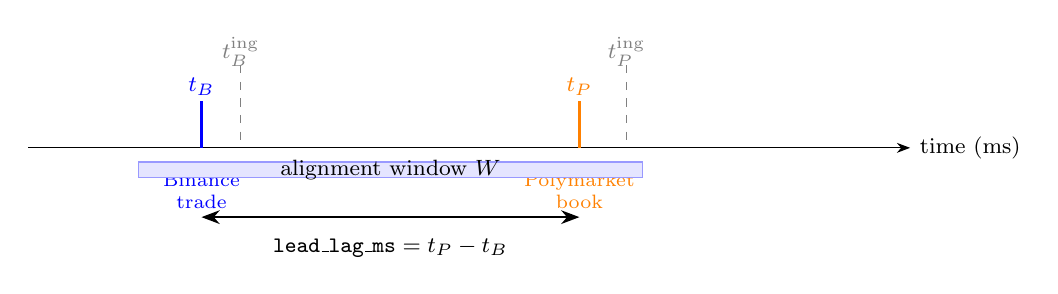
\begin{tikzpicture}[
      >=Stealth,
      font=\footnotesize,
      ts/.style={thick},
      ingest/.style={dashed, gray},
      evlabel/.style={align=center, font=\scriptsize}
    ]
    \draw[->] (0,0) -- (11.2,0) node[right] {time (ms)};

    \draw[ts, blue] (2.2,0) -- (2.2,0.6);
    \node[blue] at (2.2,0.78) {$t_B$};
    \node[blue, evlabel] at (2.2,-0.55) {Binance\\trade};
    \draw[ingest] (2.7,1.05) -- (2.7,0);
    \node[gray] at (2.7,1.22) {$t_B^{\mathrm{ing}}$};

    \draw[ts, orange] (7.0,0) -- (7.0,0.6);
    \node[orange] at (7.0,0.78) {$t_P$};
    \node[orange, evlabel] at (7.0,-0.55) {Polymarket\\book};
    \draw[ingest] (7.6,1.05) -- (7.6,0);
    \node[gray] at (7.6,1.22) {$t_P^{\mathrm{ing}}$};

    \draw[fill=blue!10, draw=blue!40] (1.4,-0.38) rectangle (7.8,-0.18);
    \node at (4.6,-0.28) {alignment window $W$};

    \draw[<->, thick] (2.2,-0.88) -- (7.0,-0.88)
      node[midway, below=4pt] {$\texttt{lead\_lag\_ms}=t_P-t_B$};
  \end{tikzpicture}
  \caption{Lead--lag pairing timeline. Source timestamps determine
    Equation~\eqref{eq:lead-lag}; ingest timestamps diagnose collector
    delay separately from cross-venue ordering.}
  \label{fig:lead-lag-timeline}
\end{figure}

Empirical lead--lag distributions on the unified split ($n=\OpenMarketLagPairs{}$;
median \OpenMarketLagMedian{}~ms) are reported in
Section~\ref{sec:exp-sync} and Figure~\ref{fig:lead-lag-hist-unified}.

\subsection{Validation Checklist}

Researchers reproducing synchronization results should:
\begin{enumerate}
  \item verify monotonicity of \texttt{source\_ts\_ms} within each stream;
  \item count duplicate payloads and reconnect gaps;
  \item plot lead--lag histograms stratified by day and market;
  \item rebuild \texttt{lag\_pairs\_ms} from raw partitions and compare checksums.
\end{enumerate}

\section{Synchronization}
\label{sec:synchronization}

Synchronization is the central technical component of OpenMarket.
For each event the recorder stores both a source timestamp (exchange-emitted)
and an ingest timestamp (collector-observed):
\begin{align}
  \texttt{source\_ts\_ms} &= \text{timestamp from the exchange or event source}, \\
  \texttt{ingest\_ts\_ms}  &= \text{timestamp when the collector received the event}.
\end{align}
Following multi-venue price-discovery practice~\cite{hasbrouck1995one},
we pair Binance and Polymarket observations inside a bounded millisecond
window and compute lead-lag as
\begin{equation}
  \texttt{lead\_lag\_ms}
    = \texttt{polymarket\_source\_ts\_ms} - \texttt{binance\_source\_ts\_ms}.
  \label{eq:lead-lag}
\end{equation}
Positive values indicate that the Polymarket event timestamp follows the
Binance event timestamp; negative values indicate the opposite.
Each pair is stored with a quality flag, Binance price, Polymarket bid,
market slug, side label, and price delta in basis points.

\subsection{Pairing and Quality Metrics}

The recorder pairs events when their source timestamps fall within a
configurable alignment window~$W$ (milliseconds).
OpenMarket treats the following as first-class dataset quality metrics,
consistent with microstructure guidance for decentralized prediction
markets~\cite{dubach2026anatomy,rahman2025sok}:
clock drift, dropped WebSocket messages, duplicate payloads, reconnect gaps,
stale order-book state, out-of-order events, and sensitivity to~$W$.

\subsection{Lead--Lag Timeline (Figure~\ref{fig:lead-lag-timeline})}

Figure~\ref{fig:lead-lag-timeline} illustrates a single matched pair.
A Binance trade arrives at source time~$t_B$; a Polymarket book update
follows at~$t_P$. Ingest times ($t_B^{\mathrm{ing}}$, $t_P^{\mathrm{ing}}$)
are shown above the axis to separate network delay from exchange-reported
ordering. The shaded interval is the alignment window~$W$.

\begin{figure}[t]
  \centering
  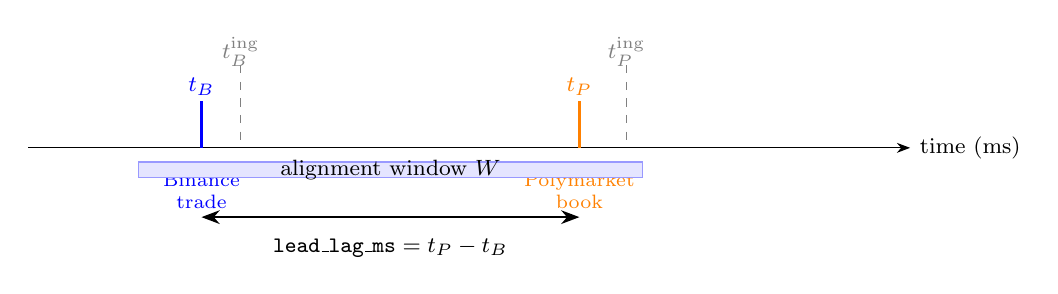
\begin{tikzpicture}[
      >=Stealth,
      font=\footnotesize,
      ts/.style={thick},
      ingest/.style={dashed, gray},
      evlabel/.style={align=center, font=\scriptsize}
    ]
    \draw[->] (0,0) -- (11.2,0) node[right] {time (ms)};

    \draw[ts, blue] (2.2,0) -- (2.2,0.6);
    \node[blue] at (2.2,0.78) {$t_B$};
    \node[blue, evlabel] at (2.2,-0.55) {Binance\\trade};
    \draw[ingest] (2.7,1.05) -- (2.7,0);
    \node[gray] at (2.7,1.22) {$t_B^{\mathrm{ing}}$};

    \draw[ts, orange] (7.0,0) -- (7.0,0.6);
    \node[orange] at (7.0,0.78) {$t_P$};
    \node[orange, evlabel] at (7.0,-0.55) {Polymarket\\book};
    \draw[ingest] (7.6,1.05) -- (7.6,0);
    \node[gray] at (7.6,1.22) {$t_P^{\mathrm{ing}}$};

    \draw[fill=blue!10, draw=blue!40] (1.4,-0.38) rectangle (7.8,-0.18);
    \node at (4.6,-0.28) {alignment window $W$};

    \draw[<->, thick] (2.2,-0.88) -- (7.0,-0.88)
      node[midway, below=4pt] {$\texttt{lead\_lag\_ms}=t_P-t_B$};
  \end{tikzpicture}
  \caption{Lead--lag pairing timeline. Source timestamps determine
    Equation~\eqref{eq:lead-lag}; ingest timestamps diagnose collector
    delay separately from cross-venue ordering.}
  \label{fig:lead-lag-timeline}
\end{figure}

Empirical lead--lag distributions on the unified split ($n=\OpenMarketLagPairs{}$;
median \OpenMarketLagMedian{}~ms) are reported in
Section~\ref{sec:exp-sync} and Figure~\ref{fig:lead-lag-hist-unified}.

\subsection{Validation Checklist}

Researchers reproducing synchronization results should:
\begin{enumerate}
  \item verify monotonicity of \texttt{source\_ts\_ms} within each stream;
  \item count duplicate payloads and reconnect gaps;
  \item plot lead--lag histograms stratified by day and market;
  \item rebuild \texttt{lag\_pairs\_ms} from raw partitions and compare checksums.
\end{enumerate}

\section{Synchronization}
\label{sec:synchronization}

Synchronization is the central technical component of OpenMarket.
For each event the recorder stores both a source timestamp (exchange-emitted)
and an ingest timestamp (collector-observed):
\begin{align}
  \texttt{source\_ts\_ms} &= \text{timestamp from the exchange or event source}, \\
  \texttt{ingest\_ts\_ms}  &= \text{timestamp when the collector received the event}.
\end{align}
Following multi-venue price-discovery practice~\cite{hasbrouck1995one},
we pair Binance and Polymarket observations inside a bounded millisecond
window and compute lead-lag as
\begin{equation}
  \texttt{lead\_lag\_ms}
    = \texttt{polymarket\_source\_ts\_ms} - \texttt{binance\_source\_ts\_ms}.
  \label{eq:lead-lag}
\end{equation}
Positive values indicate that the Polymarket event timestamp follows the
Binance event timestamp; negative values indicate the opposite.
Each pair is stored with a quality flag, Binance price, Polymarket bid,
market slug, side label, and price delta in basis points.

\subsection{Pairing and Quality Metrics}

The recorder pairs events when their source timestamps fall within a
configurable alignment window~$W$ (milliseconds).
OpenMarket treats the following as first-class dataset quality metrics,
consistent with microstructure guidance for decentralized prediction
markets~\cite{dubach2026anatomy,rahman2025sok}:
clock drift, dropped WebSocket messages, duplicate payloads, reconnect gaps,
stale order-book state, out-of-order events, and sensitivity to~$W$.

\subsection{Lead--Lag Timeline (Figure~\ref{fig:lead-lag-timeline})}

Figure~\ref{fig:lead-lag-timeline} illustrates a single matched pair.
A Binance trade arrives at source time~$t_B$; a Polymarket book update
follows at~$t_P$. Ingest times ($t_B^{\mathrm{ing}}$, $t_P^{\mathrm{ing}}$)
are shown above the axis to separate network delay from exchange-reported
ordering. The shaded interval is the alignment window~$W$.

\begin{figure}[t]
  \centering
  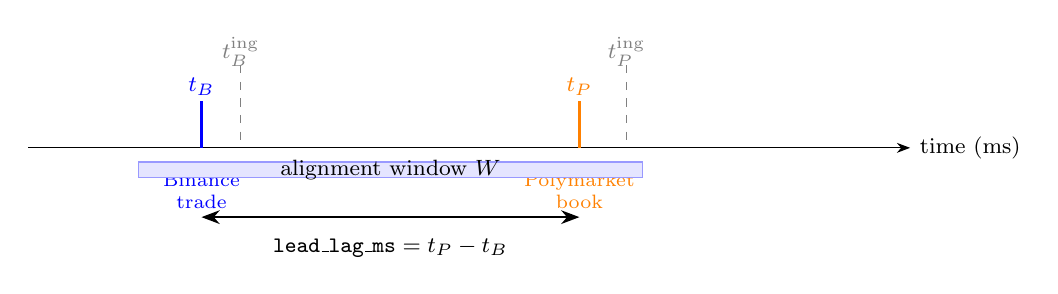
\begin{tikzpicture}[
      >=Stealth,
      font=\footnotesize,
      ts/.style={thick},
      ingest/.style={dashed, gray},
      evlabel/.style={align=center, font=\scriptsize}
    ]
    \draw[->] (0,0) -- (11.2,0) node[right] {time (ms)};

    \draw[ts, blue] (2.2,0) -- (2.2,0.6);
    \node[blue] at (2.2,0.78) {$t_B$};
    \node[blue, evlabel] at (2.2,-0.55) {Binance\\trade};
    \draw[ingest] (2.7,1.05) -- (2.7,0);
    \node[gray] at (2.7,1.22) {$t_B^{\mathrm{ing}}$};

    \draw[ts, orange] (7.0,0) -- (7.0,0.6);
    \node[orange] at (7.0,0.78) {$t_P$};
    \node[orange, evlabel] at (7.0,-0.55) {Polymarket\\book};
    \draw[ingest] (7.6,1.05) -- (7.6,0);
    \node[gray] at (7.6,1.22) {$t_P^{\mathrm{ing}}$};

    \draw[fill=blue!10, draw=blue!40] (1.4,-0.38) rectangle (7.8,-0.18);
    \node at (4.6,-0.28) {alignment window $W$};

    \draw[<->, thick] (2.2,-0.88) -- (7.0,-0.88)
      node[midway, below=4pt] {$\texttt{lead\_lag\_ms}=t_P-t_B$};
  \end{tikzpicture}
  \caption{Lead--lag pairing timeline. Source timestamps determine
    Equation~\eqref{eq:lead-lag}; ingest timestamps diagnose collector
    delay separately from cross-venue ordering.}
  \label{fig:lead-lag-timeline}
\end{figure}

Empirical lead--lag distributions on the unified split ($n=\OpenMarketLagPairs{}$;
median \OpenMarketLagMedian{}~ms) are reported in
Section~\ref{sec:exp-sync} and Figure~\ref{fig:lead-lag-hist-unified}.

\subsection{Validation Checklist}

Researchers reproducing synchronization results should:
\begin{enumerate}
  \item verify monotonicity of \texttt{source\_ts\_ms} within each stream;
  \item count duplicate payloads and reconnect gaps;
  \item plot lead--lag histograms stratified by day and market;
  \item rebuild \texttt{lag\_pairs\_ms} from raw partitions and compare checksums.
\end{enumerate}
\section{Features and Machine Learning}
\label{sec:ml}

Feature families include order-book metrics (spread, best bid/ask, microprice,
imbalance, depth, book update velocity), price metrics (returns, realized
volatility, momentum, VWAP deviation, candle shape), technical indicators (RSI,
EMA, VWAP, ATR, Bollinger Bands, MACD, ADX), and custom signals (drift score,
order-flow acceleration, scoreboard signal, whipsaw/chop detector, volume gate,
Brier calibration monitor, confidence-bin empirical edge). Features are
computed from aligned ticks and paired with settlement labels downstream.

The project includes historical Python prototypes and Rust signal code. The
legacy ML archive includes XGBoost, LightGBM, logistic meta-classifiers, SHAP
feature analysis, and stacked ensembles. The \textbf{published} binary-outcome
model uses a Rust pipeline on unified Parquet:

\begin{enumerate}
  \item \texttt{export\_step3\_from\_parquet} reads \texttt{v0.4.3-unified}
        tables and emits step3 calibration CSVs (43 features).
  \item \texttt{train\_binary\_outcome\_model} performs walk-forward logistic
        regression by market, applies Platt scaling~\cite{platt1999probabilistic},
        and writes JSON artifacts.
\end{enumerate}

On the publication workstation (Apple M5 Max), step3 export of 357{,}390 rows
across 2{,}251 markets completes in ${\sim}$63\,s; training (559 walk-forward
windows) completes in ${\sim}$67\,s. Step3 export writes 51\% of
\texttt{market\_meta} markets. The coverage audit over 4{,}450 markets reports
2{,}251 written, 1{,}241 with no Polymarket ticks in the export window, 922
with insufficient Binance trades for signal construction, 21 with missing
Binance partitions, 14 with no valid order-book snapshots after feature filters,
and one tied BTC close that is dropped because the binary label is undefined.

For public releases, model binaries are uploaded to Hugging Face Models rather
than committed to Git. The canonical \texttt{v0.2.1/} benchmark is the frozen
exported scorer evaluated on the full 357{,}390-row step3 timeline: AUC 0.841,
Brier 0.163, and ECE 0.027 (Section~\ref{sec:insights-forecast}). Because the
full timeline includes each window's training rows, this figure is an
optimistic bound; the training artifact also records the walk-forward
diagnostic (pooled OOS AUC \OpenMarketModelOosAuc{},
Brier \OpenMarketModelOosBrier{}, ECE 0.025 across 559 windows), and
Section~\ref{sec:insights-forecast} compares both against the naive mid prior
on the same rows.
Simulated positive-EV trading under 1\% fees and 0.5\% slippage yields
$-0.117$ PnL per trade. An earlier \texttt{v0.1/} pilot artifact remains for
comparison.
Reliability and per-window metrics are regenerated by
\texttt{generate\_ml\_figures.py}; forecast ablations against naive baselines
are in Section~\ref{sec:insights-forecast}.

\section{Strategy, Backtesting, and Evaluation Framework}
\label{sec:strategy}

\subsection{Strategy Archive}

The repository preserves the full evolution of the strategy line whose failure
motivated this release (v1--v15 iterations), providing historical baselines
for comparison and reproducibility. Strategies combine model confidence,
market price, entry constraints, and risk controls. The current research line includes
drift and order-flow imbalance signals, scoreboard-derived Polymarket book
signals, whipsaw/chop detection, best-signal scanning inside an entry window,
volume gating, entry price bounds, confidence and edge thresholds, Brier-score
circuit breakers, and confidence-bin empirical edge gates.

Position sizing and simulated execution assumptions are intentionally separated
from directional accuracy. Backtests report slippage, fees, assumed fill
prices, and market impact assumptions explicitly.

\subsection{Backtesting}
\label{sec:backtesting}

Backtesting processes market windows independently and evaluates entry signals
against settled outcomes under documented simulation assumptions (signal gate,
simulated fill, settlement, metric aggregation). Preferred
validation methods include walk-forward validation, rolling-window evaluation,
strict out-of-sample splits, sensitivity analysis over entry windows and
thresholds, and Monte Carlo resampling of fill and slippage assumptions. Random
row splits are discouraged because adjacent high-frequency observations are
highly autocorrelated.

\subsection{Evaluation Metrics}
\label{sec:evaluation}

Evaluation includes both predictive and simulated-economic metrics.
Economic metrics are counterfactual diagnostics under explicit fill, fee, and
slippage assumptions.

\paragraph{Predictive metrics.}
Accuracy, precision, recall, F1, ROC AUC, Brier score, and calibration
curves~\cite{brier1950verification}.

\paragraph{Simulated-economic metrics.}
Simulated win rate, expectancy, PnL, Sharpe and Sortino ratios (under stated
assumptions), maximum drawdown, turnover, average entry price, and documented
fill, fee, and slippage assumptions.

Calibration is especially important because binary market strategies are
sensitive to the difference between predicted probability and market-implied
price.

\section{Dataset}
\label{sec:dataset}

The public dataset is hosted on Hugging Face:
\url{https://huggingface.co/datasets/gregyoung14/openmarket-btc-polymarket}.

\subsection{Release Status}
\label{sec:dataset-status}

\begin{table}[t]
  \centering
  \caption{Hugging Face dataset splits (frozen at source tag \OpenMarketReleaseTag{}).}
  \label{tab:dataset-splits}
  \small
  \begin{tabular}{@{}llcp{3.8cm}@{}}
    \toprule
    Split & Version & Status & Purpose \\
    \midrule
    Unified  & \texttt{v0.4.3-unified} & Live &
      Deduped timeline (\OpenMarketTotalRows{} rows, \OpenMarketUnifiedGiB{}~GiB) \\
    Full     & \texttt{v0.2-full}        & Live &
      202-snapshot per-export archive \\
    Sample   & \texttt{v0.1-sample}      & Live &
      Schema validation, quickstart \\
    Features & \texttt{v0.4-features}    & Optional &
      One-snapshot demo; reproducible from \texttt{unified/} \\
    \bottomrule
  \end{tabular}
\end{table}

The operator archive inventories \OpenMarketSnapshots{} CDN SQLite snapshots
(\OpenMarketCollectionStart{}--\OpenMarketCollectionEnd{}). Five formerly-partial
exports were recovered with \texttt{sqlite3 .recover} and re-exported before
the final unified rebuild; queue metadata reports 202~\texttt{published-clean},
0~\texttt{published-partial}, and 0~\texttt{corrupt}.

The unified split merges overlapping \texttt{full/} exports with
\path{scripts/datasets/merge_partitions.py}, removing ${\sim}$21\% duplicate
rows. This duplicate rate is expected: each \texttt{full/} snapshot is a
point-in-time export of recorder state, so adjacent snapshots intentionally
overlap in historical rows. The unified split deduplicates those overlapping
exports by table-specific keys and timestamps rather than treating them as new
events. All splits are validated with
\path{scripts/hf/validate_sample_split.py}. Empirical statistics are regenerated
from on-disk Parquet via \texttt{analyze\_unified.py} (Section~\ref{sec:reproducibility}).

Table-level schemas and relationships are in Appendix~\ref{app:schema}.
Processed step3 features for ML are exported from unified Parquet
(\path{step3-parquet-export}) rather than shipped as a full Hugging Face split.

\begin{figure}[t]
  \centering
  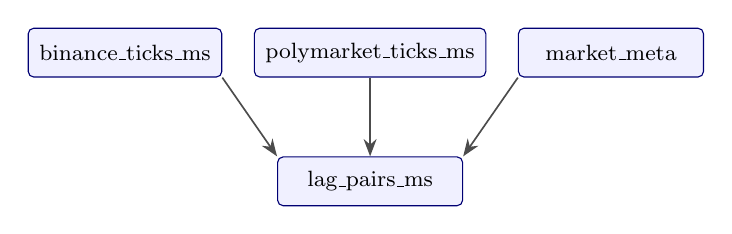
\begin{tikzpicture}[
      node distance=0.55cm and 0.4cm,
      every node/.style={narrowbox, minimum width=2.35cm}
    ]
    \node (bin) {binance\_ticks\_ms};
    \node[right=of bin] (poly) {polymarket\_ticks\_ms};
    \node[right=of poly] (meta) {market\_meta};
    \node[below=1.0cm of poly] (lag) {lag\_pairs\_ms};
    \draw[flowarr] (bin.south east) -- (lag.north west);
    \draw[flowarr] (poly) -- (lag);
    \draw[flowarr] (meta.south west) -- (lag.north east);
  \end{tikzpicture}
  \caption{Core dataset tables and relationships.}
  \label{fig:schema}
\end{figure}

\section{Experimental Characterization}
\label{sec:experiments}

We characterize the published \texttt{v0.4.3-unified} Hugging Face split with
the paper analysis scripts on local Parquet and model artifacts. Statistics below are computed from
on-disk Parquet metadata and a full scan of \texttt{lag\_pairs\_ms} (release tag
\OpenMarketReleaseTag{}). These results describe \textbf{what the archival corpus
contains}; microstructure findings and forecast benchmarks are in
Section~\ref{sec:insights}.

\subsection{Dataset Scale}
\label{sec:exp-scale}

The unified split contains \OpenMarketTotalRows{} rows across all exported tables
(Figure~\ref{fig:dataset-scale}),
occupying \OpenMarketUnifiedGiB{}~GiB on disk. The operator archive comprises
\OpenMarketSnapshots{} SQLite snapshots published from
\OpenMarketCollectionStart{} to \OpenMarketCollectionEnd{} (a 109-day
publication window). The event data inside those snapshots spans
\OpenMarketDataFirstDay{} to \OpenMarketDataLastDay{}
(\OpenMarketDataSpanDays{} calendar days), with event data on
\OpenMarketPolyObservedDays{} observed days for Polymarket and
\OpenMarketBinanceObservedDays{} for Binance; coverage is uneven, with
multi-day gaps, and no new event data was recorded after
\OpenMarketDataLastDay{} even though snapshot checkpoints
continued to be published until \OpenMarketCollectionEnd{}. After
deduplication across overlapping snapshot exports, the unified timeline removes
${\sim}$21\% duplicate rows relative to the raw \texttt{full/} union (916M
input rows $\rightarrow$ \OpenMarketTotalRows{} output rows). Most rows are
Polymarket ticks (605.6M), Binance trades (62.3M), Binance millisecond ticks
(55.8M), and explicit lag pairs (2.9M); candle tables add 498{,}525 rows and
have narrower coverage because only completed intervals are written.

\begin{figure}[t]
  \centering
  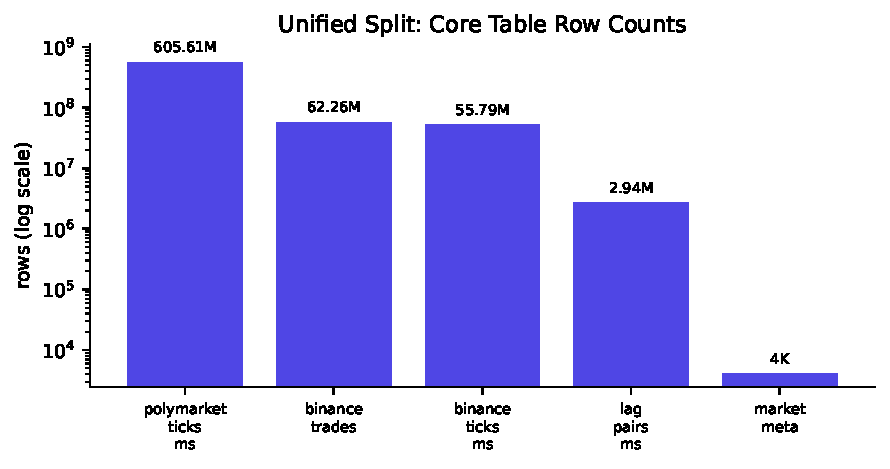
\includegraphics[width=0.92\linewidth]{dataset-scale.pdf}
  \caption{Unified split table row counts (log scale).}
  \label{fig:dataset-scale}
\end{figure}

The first five rows are the core event and metadata tables; derived candle
tables account for the remaining 498{,}525 rows in the headline total. Counts
and part numbers are tied to the frozen \texttt{v0.4.3-unified} manifest after
recovery and final deduplication; earlier draft tables generated from
pre-recovery subsets are not directly comparable.

Export quality: all \OpenMarketSnapshots{} snapshots are \texttt{published-clean}
after sqlite3 recovery of formerly-partial exports; per-snapshot export reports
document any table-level gaps.

\subsection{Synchronization Empirics}
\label{sec:exp-sync}

Lead--lag pairing produces \OpenMarketLagPairs{} matched event pairs in the
unified split. Figure~\ref{fig:lead-lag-hist-unified} shows the full distribution;
summary statistics are:

\begin{itemize}
  \item median lead--lag: \OpenMarketLagMedian{}~ms
  \item 5th / 95th percentiles: \OpenMarketLagPFive{} / \OpenMarketLagPNinetyFive{}~ms
\end{itemize}

Positive values indicate Polymarket source timestamps following Binance source
timestamps (Equation~\ref{eq:lead-lag}). On a 500k-pair sample, the recorder's
pairing-window quality flags split into \OpenMarketFlagTightPct{}\%
\texttt{tight} ($|$lag$| \le 100$~ms), \OpenMarketFlagMediumPct{}\%
\texttt{medium} ($\le 300$~ms), and \OpenMarketFlagWidePct{}\% \texttt{wide}
($> 300$~ms) pairs, so filtering to \texttt{tight} pairs retains roughly
two-thirds of the table. The long tails motivate treating
alignment-window sensitivity and clock drift as first-class quality metrics;
Section~\ref{sec:sync-clock} bounds relative clock drift empirically.

\begin{figure}[t]
  \centering
  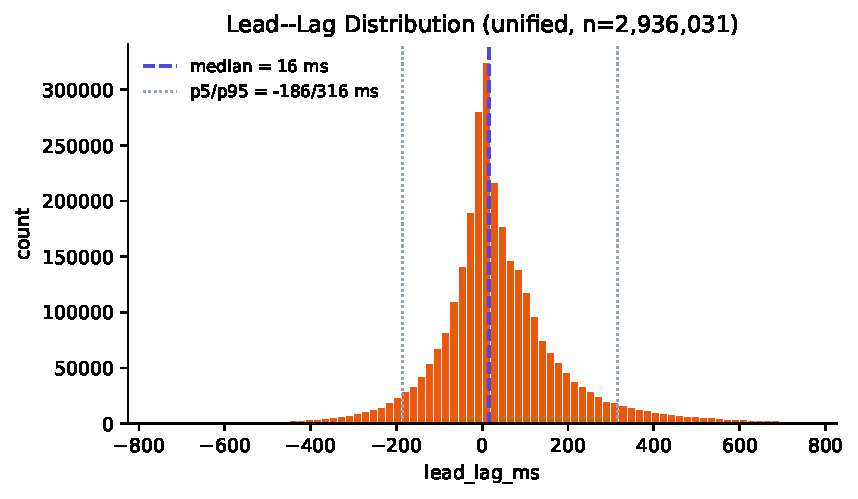
\includegraphics[width=0.88\linewidth]{lead-lag-hist.pdf}
  \caption{Empirical \texttt{lead\_lag\_ms} distribution from the unified
    \texttt{lag\_pairs\_ms} table ($n=\OpenMarketLagPairs{}$).}
  \label{fig:lead-lag-hist-unified}
\end{figure}

\subsection{Reproducibility Benchmarks}
\label{sec:exp-bench}

Environment-specific measurements on the publication workstation
(\OpenMarketHardware{}; \OpenMarketRustVersion{}) are recorded in
\texttt{assets/stats/benchmarks.json}. They include HF sample validation
(1.55\,s / 9{,}352 rows), unified Parquet metadata scan
(\OpenMarketUnifiedGiB{}~GiB in \OpenMarketUnifiedMetaScanSeconds{}\,s),
\texttt{lag\_pairs\_ms} load (\OpenMarketLagPairs{} rows in
\OpenMarketLagPairsLoadSeconds{}\,s), and the released staging backtest
(\OpenMarketBenchBacktest{}\,s across \OpenMarketBenchBacktestMarkets{}
markets). These are local I/O measurements, not cold-download benchmarks.

\section{Microstructure Findings}
\label{sec:insights}

This section reports \textbf{what we learn from the corpus}, not only what we
built. Regenerate via \texttt{analyze\_research.py} and
\texttt{analyze\_unified.py} (Section~\ref{sec:reproducibility}).

\subsection{Scale and Coverage}
\label{sec:insights-scale}

The unified archive spans 109 days and \OpenMarketTotalRows{} rows
(Table~\ref{tab:unified-rows}). Polymarket ticks dominate volume
(605.6M rows), enabling event studies at scales impractical with sample-only
public drops. After deduplicating overlapping snapshot exports, ${\sim}$21\% of
raw \texttt{full/} rows collapse---a methodological point for anyone merging
recorder archives without explicit keys.

\subsection{Lead--Lag and Cross-Venue Disagreement}
\label{sec:insights-leadlag}

Lead--lag pairs exhibit a compact median (\OpenMarketLagMedian{}~ms) but heavy
tails (5th/95th: \OpenMarketLagPFive{} / \OpenMarketLagPNinetyFive{}~ms;
Figure~\ref{fig:lead-lag-hist-unified}). Stratifying by $|$\texttt{price\_delta\_bps}$|$
quintiles shows \textbf{stable} median lead--lag (16--19~ms) across disagreement
levels (Figure~\ref{fig:lead-lag-disagreement}): cross-venue \emph{timing} does
not materially shift with contemporaneous basis-point divergence.
Disagreement regimes show the same pattern (Figure~\ref{fig:lead-lag-regime}).

Daily event volumes (Figure~\ref{fig:daily-volume}) show uneven archive
coverage without a simple ``high volume $\Rightarrow$ faster cross-venue
adjustment'' rule.
Lead--lag magnitude is uncorrelated with $|$\texttt{price\_delta\_bps}$|$
(Pearson $r \approx \OpenMarketLagPriceCorr{}$ on 500k pairs), so lag delay alone does not predict
contemporaneous mispricing magnitude.

\subsection{Polymarket Spread Stylized Facts}
\label{sec:insights-spread}

Top-of-book spreads on UP/DOWN tokens concentrate at one tick wide
(median $\approx 0.01$ probability points; 95th percentile $\approx 0.02$;
Figure~\ref{fig:spread-distribution}). Tight spreads imply that naive backtests
using mid prices can overstate executable edge---consistent with negative
simulated PnL under fees and slippage (Section~\ref{sec:ml}).

\subsection{Forecast Benchmarks and Ablations}
\label{sec:insights-forecast}

On 357{,}390 step3 rows exported from unified Parquet, we score the frozen
\texttt{v0.2.1} artifact and simple forecast baselines
(Table~\ref{tab:forecast-benchmarks}, Figure~\ref{fig:forecast-benchmarks}).
All metrics are computed by \texttt{analyze\_research.py}; expected calibration
error (ECE) uses 10 equal-width probability bins.

\begin{table}[t]
  \centering
  \caption{Forecast benchmarks on step3 rows (full timeline). Lower is better
    for Brier, ECE, and log loss.}
  \label{tab:forecast-benchmarks}
  \small
  \begin{tabular}{@{}lrrrrr@{}}
    \toprule
    Model & AUC & Brier & ECE & Log loss & $\mu$s/row \\
    \midrule
    Naive \texttt{market\_mid\_prior\_up} & 0.840 & 0.163 & 0.014 & 0.486 & -- \\
    Logistic + Platt (\texttt{v0.2.1})    & 0.841 & 0.163 & \OpenMarketLogisticEce{} & 0.489 & \OpenMarketLogisticScoreUs{} \\
    \texttt{drift\_prob\_up} only         & 0.773 & 0.218 & 0.145 & 0.792 & -- \\
    \texttt{imbalance\_60s} (sigmoid)     & 0.586 & 0.246 & 0.031 & 0.685 & -- \\
    \bottomrule
  \end{tabular}
\end{table}

\textbf{Effect size.} Logistic \texttt{v0.2.1} beats the naive mid prior by
$\Delta$AUC $= \OpenMarketAucDiff{}$ (paired bootstrap 95\% CI
$[\OpenMarketAucDiffLow{}, \OpenMarketAucDiffHigh{}]$; one-sided
$p < 0.001$, $n=357{,}390$). The lift is statistically
detectable but \emph{economically} tiny relative to fees and spread---hence
negative simulated PnL. The market prior is also better calibrated
(ECE \OpenMarketNaiveEce{} vs.\ \OpenMarketLogisticEce{}), so the logistic
model should be read as a marginal ranking improvement, not a replacement for
market-implied probability.

\textbf{Spread and reliability.} At one-tick spreads ($\leq 0.011$), Brier is
$\approx \OpenMarketBrierTight{}$; at wider quotes ($\geq 0.015$), Brier rises to
$\approx \OpenMarketBrierWide{}$. Realized-volatility terciles show a parallel
gradient (0.159 high-vol vs.\ 0.164 low-vol): forecasts are more reliable when
underlying BTC activity is elevated and degrade when Polymarket quotes widen.

\textbf{Takeaway.} Multivariate features add marginal ranking skill over the
Polymarket mid; drift alone is weaker; raw order-flow imbalance fails without
context; and the strongest published baseline remains economically dominated by
fees, spread, and calibration error. These are diagnostic baselines the
infrastructure enables at 357k-row scale in minutes on a laptop---not a claim
of tradable alpha.

\begin{figure}[t]
  \centering
  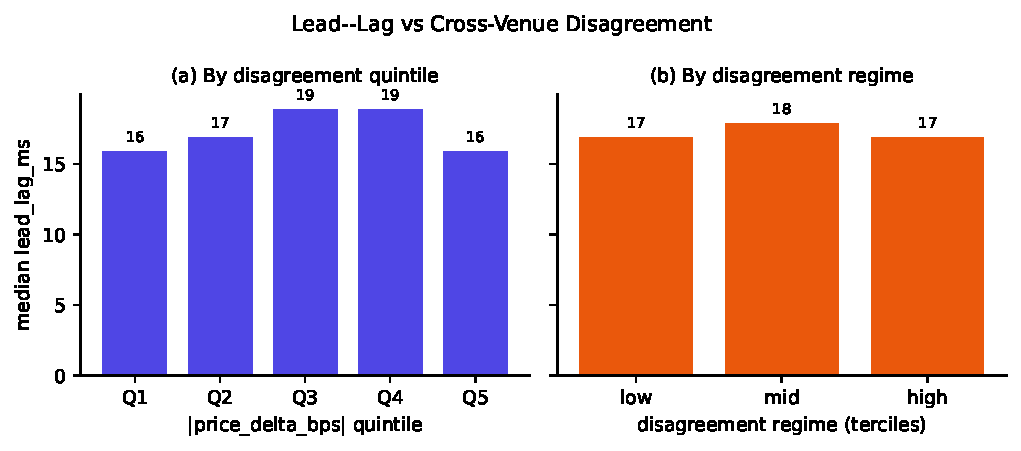
\includegraphics[width=0.88\linewidth]{lead-lag-vs-disagreement.pdf}
  \caption{Median lead--lag by $|$\texttt{price\_delta\_bps}$|$ quintile
    (\texttt{lag\_pairs\_ms}, 500k subsample).}
  \label{fig:lead-lag-disagreement}
\end{figure}

\begin{figure}[t]
  \centering
  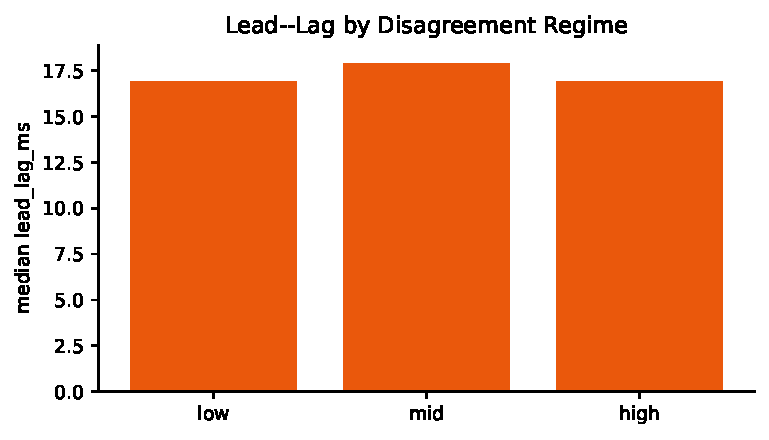
\includegraphics[width=0.82\linewidth]{lead-lag-by-regime.pdf}
  \caption{Median lead--lag by cross-venue disagreement regime (terciles of
    $|$\texttt{price\_delta\_bps}$|$).}
  \label{fig:lead-lag-regime}
\end{figure}

\begin{figure}[t]
  \centering
  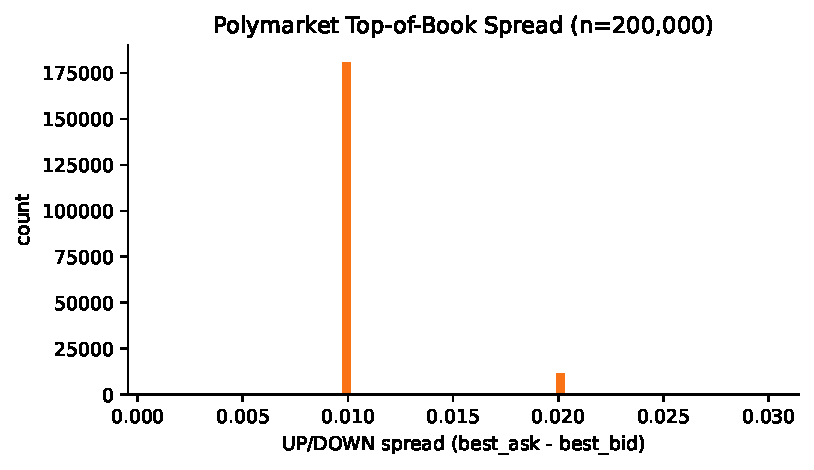
\includegraphics[width=0.88\linewidth]{spread-distribution.pdf}
  \caption{Polymarket top-of-book spread distribution (200k tick subsample).}
  \label{fig:spread-distribution}
\end{figure}

\begin{figure}[t]
  \centering
  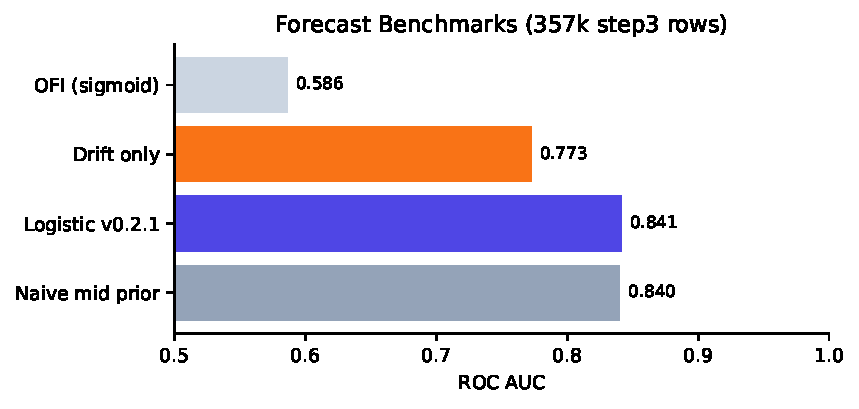
\includegraphics[width=0.92\linewidth]{forecast-benchmarks.pdf}
  \caption{Forecast benchmark ROC AUC on step3 rows.}
  \label{fig:forecast-benchmarks}
\end{figure}

\section{Reproducibility}
\label{sec:reproducibility}

OpenMarket treats reproducibility as a first-class systems requirement. Any
benchmark, backtest, or paper result should be reconstructible from: source
commit (Git SHA), dataset version (HF revision or snapshot manifest hash), model
version (or \texttt{none}), config file, exact command line, and random seed.

\subsection{Build Verification}

\begin{lstlisting}[language=bash]
git clone https://github.com/gregyoung14/openmarket.git
cd openmarket
cargo check --workspace
\end{lstlisting}

\subsection{Fast Path (Hugging Face Sample Split)}

\begin{lstlisting}[language=bash]
python3 -m venv .venv
.venv/bin/pip install -r scripts/datasets/requirements.txt \
                     -r scripts/hf/requirements.txt
.venv/bin/python scripts/hf/validate_sample_split.py
.venv/bin/python scripts/hf/benchmark_baseline.py
\end{lstlisting}

\subsection{Full Reproduction (Unified HF Split)}

\begin{lstlisting}[language=bash]
.venv/bin/python datasets/download.py --split unified --out data/hf_cache
\end{lstlisting}

\subsection{ML Model Reproduction (Rust)}

\begin{lstlisting}[language=bash]
cargo build -p step3-parquet-export -p binary-outcome-trainer --release
./target/release/export_step3_from_parquet \
  --parquet-root data/hf_release/unified_parquet \
  --out-dir data/hf_release/features_exports
./target/release/train_binary_outcome_model \
  --input data/hf_release/features_exports/step3_binary_calibration_<ts>.csv \
  --artifact-dir data/ml_artifacts
\end{lstlisting}

Regenerate paper statistics and figures:

\begin{lstlisting}[language=bash]
cd paper
./scripts/compile.sh
# or individually:
.venv/bin/python scripts/paper/analyze_unified.py \
  --root ../data/hf_release/unified_parquet
.venv/bin/python scripts/paper/analyze_research.py
.venv/bin/python scripts/paper/generate_ml_figures.py
\end{lstlisting}

Legacy operator SQLite snapshots remain available for migration only.

\subsection{Docker Reproduction}

\begin{lstlisting}[language=bash]
cp configs/openmarket.example.env .env
docker compose -f docker/docker-compose.yml up
\end{lstlisting}

\subsection{Required Reporting Metadata}

Each published result should report CPU model, RAM, storage type, OS, Rust and
Python versions, dataset version, model version, config file, command, and random
seed.

\begin{figure}[t]
  \centering
  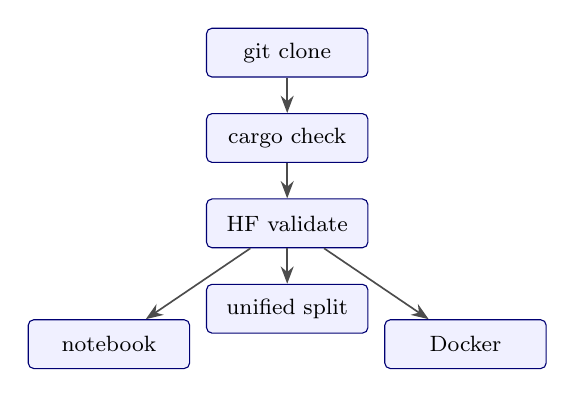
\begin{tikzpicture}[
      node distance=0.45cm and 0.9cm,
      every node/.style={narrowbox}
    ]
    \node (clone) {git clone};
    \node[below=of clone] (check) {cargo check};
    \node[below=of check] (valid) {HF validate};
    \node[below left=0.9cm and 0.2cm of valid] (nb) {notebook};
    \node[below=of valid] (uni) {unified split};
    \node[below right=0.9cm and 0.2cm of valid] (dock) {Docker};
    \draw[flowarr] (clone) -- (check);
    \draw[flowarr] (check) -- (valid);
    \draw[flowarr] (valid) -- (nb);
    \draw[flowarr] (valid) -- (uni);
    \draw[flowarr] (valid) -- (dock);
  \end{tikzpicture}
  \caption{Reproducibility flow: clone, validate, then optional notebook, full
    split, or Docker stack.}
  \label{fig:repro}
\end{figure}
\section{Discussion}
\label{sec:discussion}

\subsection{What This Enables That Prior Work Does Not}

Dubach~\cite{dubach2026anatomy} establishes Polymarket microstructure stylized
facts on tick data; Saguillo et al.~\cite{saguillo2025arbitrage} quantify
arbitrage gaps. Neither provides a reproducible \textbf{Binance--Polymarket}
timeline with published pairing metadata and walk-forward calibration baselines.
OpenMarket lowers the cost of questions such as:
\begin{itemize}
  \item How stable is lead--lag across volatility/disagreement regimes?
  \item Does Polymarket mid probability subsume external drift signals?
  \item How sensitive are calibration metrics to fees, spreads, and pairing
        window~$W$?
\end{itemize}
Section~\ref{sec:insights} gives initial answers; the tooling is the enduring
contribution.

\subsection{Positioning for Venues}

The paper is best read as a \textbf{data-and-methods} release with empirical
baselines---appropriate for arXiv, ML-for-finance workshops, or data-descriptor
journals---rather than as a pure systems or pure econometrics theory paper. We
embrace that framing: the field needs public corpora and honest negative results
as much as novel alpha claims.

\subsection{Domain Generalizability}

BTC 15-minute markets are a high-activity microcosm of Polymarket CLOB trading:
useful for synchronization methodology and short-horizon forecasting baselines,
but not representative of slower political or macro markets. Extensions to other
assets should preserve source/ingest timestamps and publish pairing metadata the
way this release does.

\subsection{Operational and Regulatory Context}

Polygon settlement latency, oracle definition risk, and U.S.\ regulatory
uncertainty affect economic interpretation but are outside our artifact. We
document collector-host clock drift and WebSocket gaps; users should not treat
top-of-book backtests as executable PnL without explicit queue and fee models.

\subsection{Data Availability and Ethics}

The Hugging Face corpus contains only public market data (order books, trades,
metadata) collected from open APIs---no user identities or private positions.
The GitHub repository ships under Apache~2.0; dataset and model cards document
licenses and version pins. Cite the dataset version and source tag
(\OpenMarketReleaseTag{}) in derivative work (see repository \path{CITATION.md}).

\subsection{Limitations and Extensions}

Step3 export writes ${\sim}$50\% of \texttt{market\_meta} markets (missing ticks
or trades). Full \texttt{features/} Parquet is not on Hugging Face; researchers
should run \path{export_step3_from_parquet} locally. Community extensions
(neural sequence models, additional assets, benchmark leaderboards) can build on
the frozen \OpenMarketReleaseTag{} tag without implying ongoing maintenance.
\section{Limitations}
\label{sec:limitations}

\textbf{Domain scope.} BTC 15-minute Polymarket binaries are a niche but liquid
regime: high tick rate, tight spreads, and volatile underlying spot. Stylized
facts and benchmarks here may not transfer to election markets, long-dated
events, or illiquid books without re-collection and re-calibration.

\textbf{Data and methods.} WebSocket outages can create gaps; collector clocks
can drift; top-of-book backtests may overstate execution quality; mishandled
settlement labels can leak information; step3 export covers ${\sim}$50\% of
\texttt{market\_meta} markets; full-archive \texttt{features/} Parquet is not
on Hugging Face (run \path{export_step3_from_parquet} locally).

\textbf{Model comparisons.} The repository contains legacy XGBoost, LightGBM,
stacking, and SHAP prototypes, but these were exploratory strategy artifacts,
not frozen benchmarks on the unified \texttt{v0.4.3} step3 export. The main
paper therefore reports only baselines regenerated from the archived release.
Direct tree-model, neural sequence, and market-by-market benchmark suites remain
future work.

\textbf{Live trading.} Simulated outcomes are sensitive to regime and fee
assumptions; live execution adds latency, queue position, partial fills, and
regulatory uncertainty not modeled in this artifact.

\section{Conclusion}
\label{sec:conclusion}

We presented OpenMarket, an open-source pipeline and, to our knowledge, the
first public millisecond-level Polymarket BTC / Binance BTC-USDT paired corpus
with explicit pairing metadata. The release includes \OpenMarketTotalRows{}
deduplicated rows, \OpenMarketLagPairs{} lead--lag pairs, reproducible Rust
exporters and trainers, and Hugging Face artifacts
(\texttt{v0.4.3-unified}, \texttt{v0.2.1/} model).

Initial analyses show tight Polymarket spreads, heavy-tailed lead--lag with a
compact median, and forecast benchmarks where a walk-forward logistic model
matches but does not beat the naive mid prior out-of-sample---useful negative
and null results for the community. We invite researchers to use the corpus for microstructure and
forecasting studies, extend the tooling to new venues, and cite the dataset
version used in each experiment.


\section*{Funding and Competing Interests}
This project was produced as an independent open-source release. The author
declares no external funding and no competing interests.

\bibliography{bibliography}

\end{document}
